\documentclass{article}
\usepackage{graphicx} %package to manage images
\usepackage[utf8]{inputenc}
\usepackage[a4paper, total={6in, 8in}]{geometry}
\usepackage{xurl}
\usepackage{hyperref}
\usepackage{float}
\title{Relatório 16 \\ Proporções e critério de inclusão}
\author{Pedro A. S. O. Neto}
\date{Novembro, 2022}

\begin{document}

\maketitle

\section{Proporções e cutoffs}

Analisamos a proporção entre tempo de fixação e duração total do vídeo por participante e trial. Valores próximos de 1 indicam que o participante tem fixações que duram próximo do tempo total do vídeo. Proporções 0 indicam que o participante não teve fixações durante o vídeo (Figura 1).

\begin{figure}[]
  \caption{Distribuição geral de proporções por vídeo}
  \noindent\makebox[\textwidth]{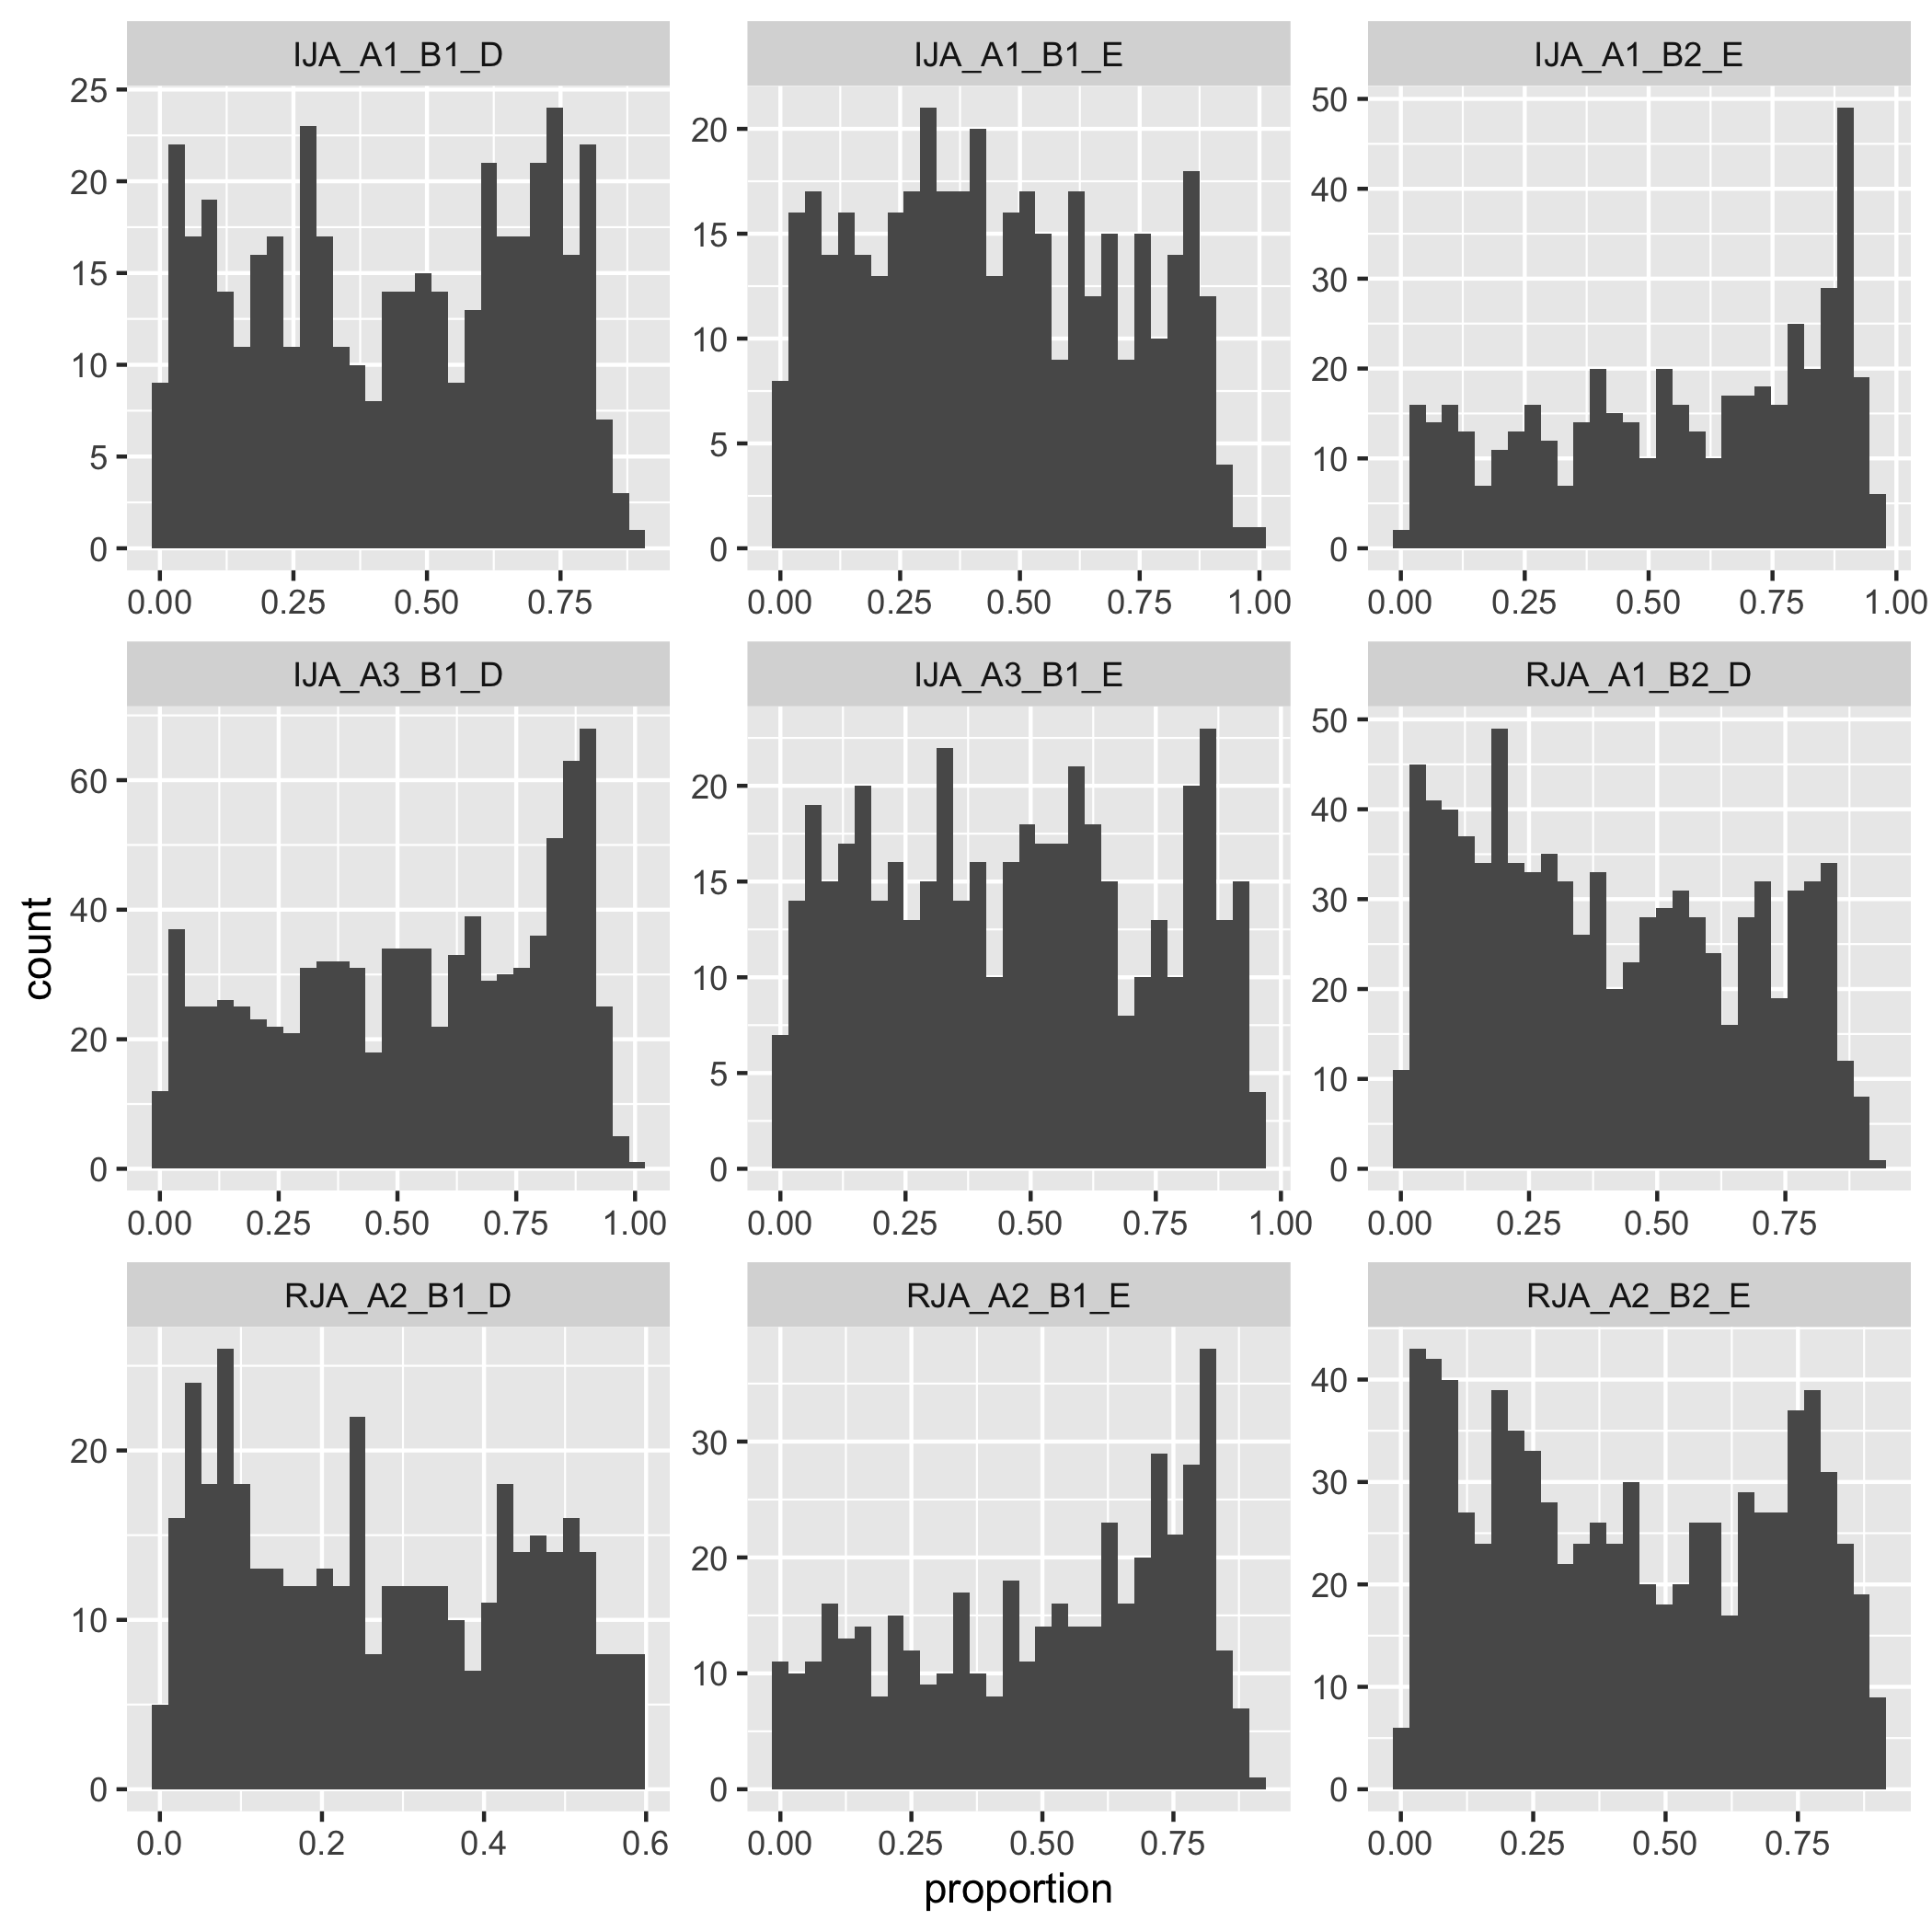
\includegraphics[scale=0.2]{./generalDistribution.png}}
  \centering
\end{figure}

Proporções de fixação podem ser usadas como critério de inclusão/exclusão de participantes (e.g., são incluidas apenas trials onde o participante apresenta uma proporção de fixações de $0.5$ ou mais). Nas próximas seções deste relatório, eu apresento simulações de diferentes níveis de threshold.

\section{Simulações}

A Tabela 1 apresenta, em proporção, o número de participantes (N\_left) e o número de trials (n\_trials) restantes após a aplicação de diferentes níveis de threshold (treshold).

\begin{table}[ht]
\centering
\begin{tabular}{rrrr}
  \hline
 & N\_left & n\_trials & threshold \\
  \hline
1 & 0.63 & 0.20 & 0.75 \\
  2 & 0.87 & 0.45 & 0.50 \\
  3 & 0.95 & 0.71 & 0.25 \\
  4 & 0.98 & 0.82 & 0.15 \\
   \hline
\end{tabular}
\end{table}


\end{document}
